% ============================================================
%  REPORTE FINAL — Reconocimiento de Patrones
%  Universidad Tecnológica de la Mixteca (UTM)
%  Alumno: José Ramón Aragón Toledo
% ============================================================
\documentclass[12pt, letterpaper]{article}

% ----- Codificación y lenguaje -----
\usepackage[utf8]{inputenc}
\usepackage[T1]{fontenc}
\usepackage[spanish, es-nodecimaldot]{babel}

% ----- Márgenes -----
\usepackage[top=2.5cm, bottom=2.5cm, left=3cm, right=2.5cm]{geometry}

% ----- Tipografía -----
\usepackage{lmodern}

% ----- Tablas -----
\usepackage{booktabs}
\usepackage{array}
\usepackage{multirow}
\usepackage{xcolor}
\usepackage{colortbl}

% ----- Figuras -----
\usepackage{graphicx}
\usepackage{float}

% ----- Interlineado -----
\usepackage{setspace}
\onehalfspacing

% ----- Matemáticas -----
\usepackage{amsmath}

% ----- Cabecera y pie de página -----
\usepackage{fancyhdr}
\pagestyle{fancy}
\fancyhf{}
\fancyhead[L]{\small Reconocimiento de Patrones}
\fancyhead[R]{\small UTM — Instituto de Computación}
\fancyfoot[C]{\thepage}
\renewcommand{\headrulewidth}{0.4pt}

% ----- Hipervínculos -----
\usepackage[hidelinks]{hyperref}

% ----- Colores para tablas -----
\definecolor{rowgray}{gray}{0.93}
\definecolor{headerblue}{RGB}{68, 114, 196}

% ============================================================
\begin{document}

% ============================================================
%  PORTADA
% ============================================================
\begin{titlepage}
    \centering
    \vspace*{1cm}

    {\Large \textbf{Universidad Tecnológica de la Mixteca}}\\[0.3cm]
    {\large Instituto de Computación}\\[0.2cm]
    {\large Ingeniería en Computación}

    \vspace{1.5cm}
    \rule{\linewidth}{0.6pt}\\[0.5cm]
    {\LARGE \textbf{Clasificación de Niveles de Ansiedad, Estrés\\[0.2cm]
    y Depresión mediante Modelos de\\[0.2cm]
    Bayes Ingenuo y Árboles de Decisión}}\\[0.5cm]
    \rule{\linewidth}{0.6pt}

    \vspace{1.5cm}
    {\large \textbf{Materia:} Reconocimiento de Patrones}\\[1cm]

    \vspace{1cm}
    {\large \textbf{Alumno:}}\\[0.4cm]
    {\Large José Ramón Aragón Toledo}

    \vfill
    {\large Huajuapan de León, Oaxaca \hfill Abril, 2026}
\end{titlepage}

% ============================================================
%  ÍNDICE
% ============================================================
\tableofcontents
\newpage

% ============================================================
\section{Introducción}
% ============================================================

El bienestar mental estudiantil es un área de creciente interés en sistemas
educativos a nivel mundial. La detección temprana de niveles elevados de
ansiedad, estrés y depresión puede permitir intervenciones oportunas que
mejoren el rendimiento académico y la calidad de vida de los estudiantes.

El presente reporte documenta el proceso completo de clasificación multiclase
aplicado al conjunto de datos \textit{StressLevelDataset.csv}, el cual
comprende \textbf{1\,100 registros} de estudiantes con \textbf{20 variables}
de naturaleza fisiológica, psicológica, social y ambiental. La variable
objetivo principal es \texttt{stress\_level}, codificada en tres clases:
\textbf{Bajo (0)}, \textbf{Medio (1)} y \textbf{Alto (2)}.

Los objetivos del proyecto son:

\begin{enumerate}
    \item Construir modelos de clasificación usando \textit{Gaussian Naive Bayes}
          y \textit{Decision Tree Classifier} con todas las variables disponibles
          (\textbf{Tarea 1}).
    \item Aplicar selección de características mediante \textbf{Información Mutua
          (MMI)} y comparar el desempeño con el subconjunto reducido
          (\textbf{Tarea 2}).
    \item Identificar los predictores más relevantes para los niveles de
          \textbf{ansiedad} y \textbf{depresión} mediante el análisis de los
          rankings obtenidos.
\end{enumerate}

Todos los experimentos se implementaron con \texttt{Python 3.12} y la
biblioteca \texttt{scikit-learn 1.8}, garantizando reproducibilidad mediante
\texttt{random\_state = 42}.

% ============================================================
\section{Preprocesamiento de Datos}
% ============================================================

\subsection{Carga y verificación de calidad}

El conjunto de datos fue inspeccionado formalmente con la biblioteca
\texttt{pandas}. Los resultados de la auditoría de calidad se resumen a
continuación:

\begin{itemize}
    \item \textbf{Valores nulos:} 0 en las 21 columnas (20 variables +
          1 objetivo).
    \item \textbf{Filas duplicadas:} 0.
    \item \textbf{Tipos de datos:} todos enteros (\texttt{int64}), sin
          requerir codificación adicional.
\end{itemize}

\subsection{Distribución de la variable objetivo}

La Tabla~\ref{tab:distribucion} muestra que las tres clases presentan una
distribución prácticamente uniforme ($\approx\!33\%$ cada una), condición
que garantiza que los modelos no estén sesgados por desbalance de clases.

\begin{table}[H]
    \centering
    \caption{Distribución de la variable objetivo \texttt{stress\_level}}
    \label{tab:distribucion}
    \begin{tabular}{lcc}
        \toprule
        \textbf{Clase} & \textbf{Frecuencia} & \textbf{Porcentaje (\%)} \\
        \midrule
        \rowcolor{rowgray} Bajo (0)  & 373 & 33.91 \\
                           Medio (1) & 358 & 32.55 \\
        \rowcolor{rowgray} Alto (2)  & 369 & 33.55 \\
        \midrule
        \textbf{Total} & 1\,100 & 100.00 \\
        \bottomrule
    \end{tabular}
\end{table}

\subsection{Discretización por Ancho Constante (\textit{Equal Width})}

Previo al análisis de selección de características, las variables
\texttt{anxiety\_level}, \texttt{self\_esteem} y \texttt{depression} fueron
discretizadas mediante el método de \textbf{Ancho Constante} (\textit{Equal
Width Binning}), el cual divide el rango continuo de cada variable en $k$
intervalos de igual amplitud. Este paso tiene dos objetivos:

\begin{enumerate}
    \item Reducir el ruido en variables con alta variabilidad dentro de una
          misma clase.
    \item Hacer explícita la naturaleza ordinal de estas variables, lo que
          mejora la estimación de la Información Mutua en pasos posteriores.
\end{enumerate}

Para cada variable $X$ con rango $[X_{\min}, X_{\max}]$ y $k$ intervalos,
el ancho de cada bin se calcula como:

\begin{equation}
    w = \frac{X_{\max} - X_{\min}}{k}
\end{equation}

\subsection{Escalado y división de datos}

Se aplicó \textbf{StandardScaler} para normalizar las escalas de las
características, transformando cada variable a media~$\mu = 0$ y desviación
estándar $\sigma = 1$:

\begin{equation}
    z = \frac{x - \mu}{\sigma}
\end{equation}

El escalador se ajustó \emph{únicamente} sobre el conjunto de entrenamiento
y se aplicó a ambos conjuntos para evitar fuga de información
(\textit{data leakage}).

La división \textbf{Hold-out} se realizó con los parámetros de la
Tabla~\ref{tab:split}.

\begin{table}[H]
    \centering
    \caption{Parámetros y resultados del split Hold-out}
    \label{tab:split}
    \begin{tabular}{lcc}
        \toprule
        \textbf{Parámetro} & \textbf{Valor} & \textbf{Muestras} \\
        \midrule
        \rowcolor{rowgray} Entrenamiento & 70\% & 770 \\
        Prueba         & 30\% & 330 \\
        \rowcolor{rowgray} \texttt{random\_state} & 42 & --- \\
        \texttt{stratify} & \texttt{y} & --- \\
        \bottomrule
    \end{tabular}
\end{table}

% ============================================================
\section{Metodología de Clasificación — Tarea 1}
% ============================================================

\subsection{Modelos utilizados}

Se entrenaron dos algoritmos de clasificación con las \textbf{20 variables}
completas del dataset:

\begin{itemize}
    \item \textbf{Gaussian Naive Bayes} (\texttt{GaussianNB}): clasificador
          probabilístico basado en el teorema de Bayes que asume independencia
          condicional entre características y distribución gaussiana por
          clase. Su fortaleza radica en su eficiencia computacional y su
          buen desempeño incluso con datos de tamaño moderado.

    \item \textbf{Decision Tree Classifier} con \texttt{max\_depth = 6}:
          árbol de decisión cuya profundidad máxima fue acotada para
          controlar el sobreajuste (\textit{overfitting}), favoreciendo la
          generalización sobre el conjunto de prueba.
\end{itemize}

\subsection{Resultados — Tarea 1}

La Tabla~\ref{tab:tarea1} presenta las métricas de evaluación ponderadas
por clase obtenidas sobre el 30\% de datos de prueba.

\begin{table}[H]
    \centering
    \caption{Métricas de clasificación — Tarea 1 (20 variables)}
    \label{tab:tarea1}
    \begin{tabular}{lcccc}
        \toprule
        \textbf{Modelo} & \textbf{Accuracy} & \textbf{Precision} &
        \textbf{Recall} & \textbf{F1-Score} \\
        \midrule
        \rowcolor{rowgray}
        Gaussian Naive Bayes      & 88.18\% & 0.8990 & 0.8818 & 0.8837 \\
        Decision Tree (depth=6)   & 88.48\% & 0.8853 & 0.8848 & 0.8849 \\
        \bottomrule
    \end{tabular}
\end{table}

Ambos modelos superan el \textbf{88\%} de exactitud, confirmando la alta
separabilidad de las clases en este conjunto de datos. Un hallazgo destacado
es que el modelo Gaussian Naive Bayes alcanzó un \textbf{Recall = 0.96}
para la clase \textit{Alto (2)}, identificando correctamente el 96\% de los
casos de estrés elevado, propiedad especialmente valiosa en contextos de
detección temprana.

\subsection{Matrices de Confusión}

\begin{table}[H]
    \centering
    \caption{Matriz de Confusión — Gaussian Naive Bayes (Tarea 1)}
    \label{tab:cm_gnb}
    \begin{tabular}{lccc}
        \toprule
        \textbf{Real $\backslash$ Predicho} & \textbf{Bajo (0)} &
        \textbf{Medio (1)} & \textbf{Alto (2)} \\
        \midrule
        \rowcolor{rowgray} Bajo (0)  &  94 &  0 & 18 \\
                           Medio (1) &   3 & 90 & 14 \\
        \rowcolor{rowgray} Alto (2)  &   4 &  0 & 107 \\
        \bottomrule
    \end{tabular}
\end{table}

\begin{table}[H]
    \centering
    \caption{Matriz de Confusión — Decision Tree (Tarea 1)}
    \label{tab:cm_dt}
    \begin{tabular}{lccc}
        \toprule
        \textbf{Real $\backslash$ Predicho} & \textbf{Bajo (0)} &
        \textbf{Medio (1)} & \textbf{Alto (2)} \\
        \midrule
        \rowcolor{rowgray} Bajo (0)  & 98 &  5 &  9 \\
                           Medio (1) &  5 & 95 &  7 \\
        \rowcolor{rowgray} Alto (2)  &  6 &  6 & 99 \\
        \bottomrule
    \end{tabular}
\end{table}

% ============================================================
\section{Selección de Características — Tarea 2}
% ============================================================

\subsection{Información Mutua (MMI)}

La \textbf{Información Mutua} cuantifica la dependencia estadística entre
una variable aleatoria $X$ y la variable objetivo $Y$, capturando tanto
relaciones lineales como no lineales:

\begin{equation}
    I(X;\,Y) = \sum_{y \in Y}\sum_{x \in X}
    p(x,y)\,\log\!\left(\frac{p(x,y)}{p(x)\,p(y)}\right)
\end{equation}

Un valor $I(X;Y) = 0$ indica independencia estadística, mientras que
valores mayores indican mayor capacidad predictiva de $X$ sobre $Y$. Se
calculó mediante \texttt{mutual\_info\_classif} de \texttt{scikit-learn},
ajustado \emph{únicamente} sobre el conjunto de entrenamiento.

\subsection{Contraste con el Factor de Fisher}

Para validar la selección, los resultados de MMI se contrastaron con el
\textbf{Factor de Fisher} (ANOVA F-value), que cuantifica la separación
entre medias de clase en función de la varianza intra-clase:

\begin{equation}
    F = \frac{\text{Varianza entre clases}}{\text{Varianza intra-clase}}
\end{equation}

La comparación reveló que ambos métodos coinciden en \textbf{3 de las 5}
primeras posiciones. La principal discrepancia es \texttt{academic\_performance}
(Fisher: posición 4, MMI: posición 13), lo que indica que esta variable
tiene una separación lineal de medias alta pero baja capacidad discriminante
no lineal. Dado que el dataset tiene variables discretas y ordinales, se
concluye que \textbf{MMI es el criterio más adecuado} para este tipo de
datos.

\subsection{Ranking MMI — Ansiedad y Depresión}

La Tabla~\ref{tab:ranking_mmi} presenta el Top~5 de variables más
informativas para los targets \texttt{anxiety\_level} y \texttt{depression}.

\begin{table}[H]
    \centering
    \caption{Top 5 — Ranking MMI por target}
    \label{tab:ranking_mmi}
    \begin{tabular}{clcc}
        \toprule
        \textbf{Pos.} & \textbf{Característica} &
        \textbf{MI (Ansiedad)} & \textbf{MI (Depresión)} \\
        \midrule
        \rowcolor{rowgray}
        1 & blood\_pressure               & 0.7473 & 0.7977 \\
        2 & bullying                      & 0.7193 & --- \\
        \rowcolor{rowgray}
        3 & sleep\_quality                & 0.6981 & 0.7209 \\
        4 & future\_career\_concerns      & --- & --- \\
        \rowcolor{rowgray}
        5 & self\_esteem                  & --- & --- \\
        \midrule
        2 (Dep.) & sleep\_quality         & --- & 0.7209 \\
        \rowcolor{rowgray}
        3 (Dep.) & anxiety\_level         & --- & 0.6935 \\
        \bottomrule
    \end{tabular}
\end{table}

Las figuras \ref{fig:mmi_anxiety} y \ref{fig:mmi_depression} muestran el
ranking completo de las 19 variables para cada target, ordenadas de mayor
a menor importancia.

% ── Figura 1: Ansiedad ──────────────────────────────────────────────────────
\begin{figure}[H]
    \centering
    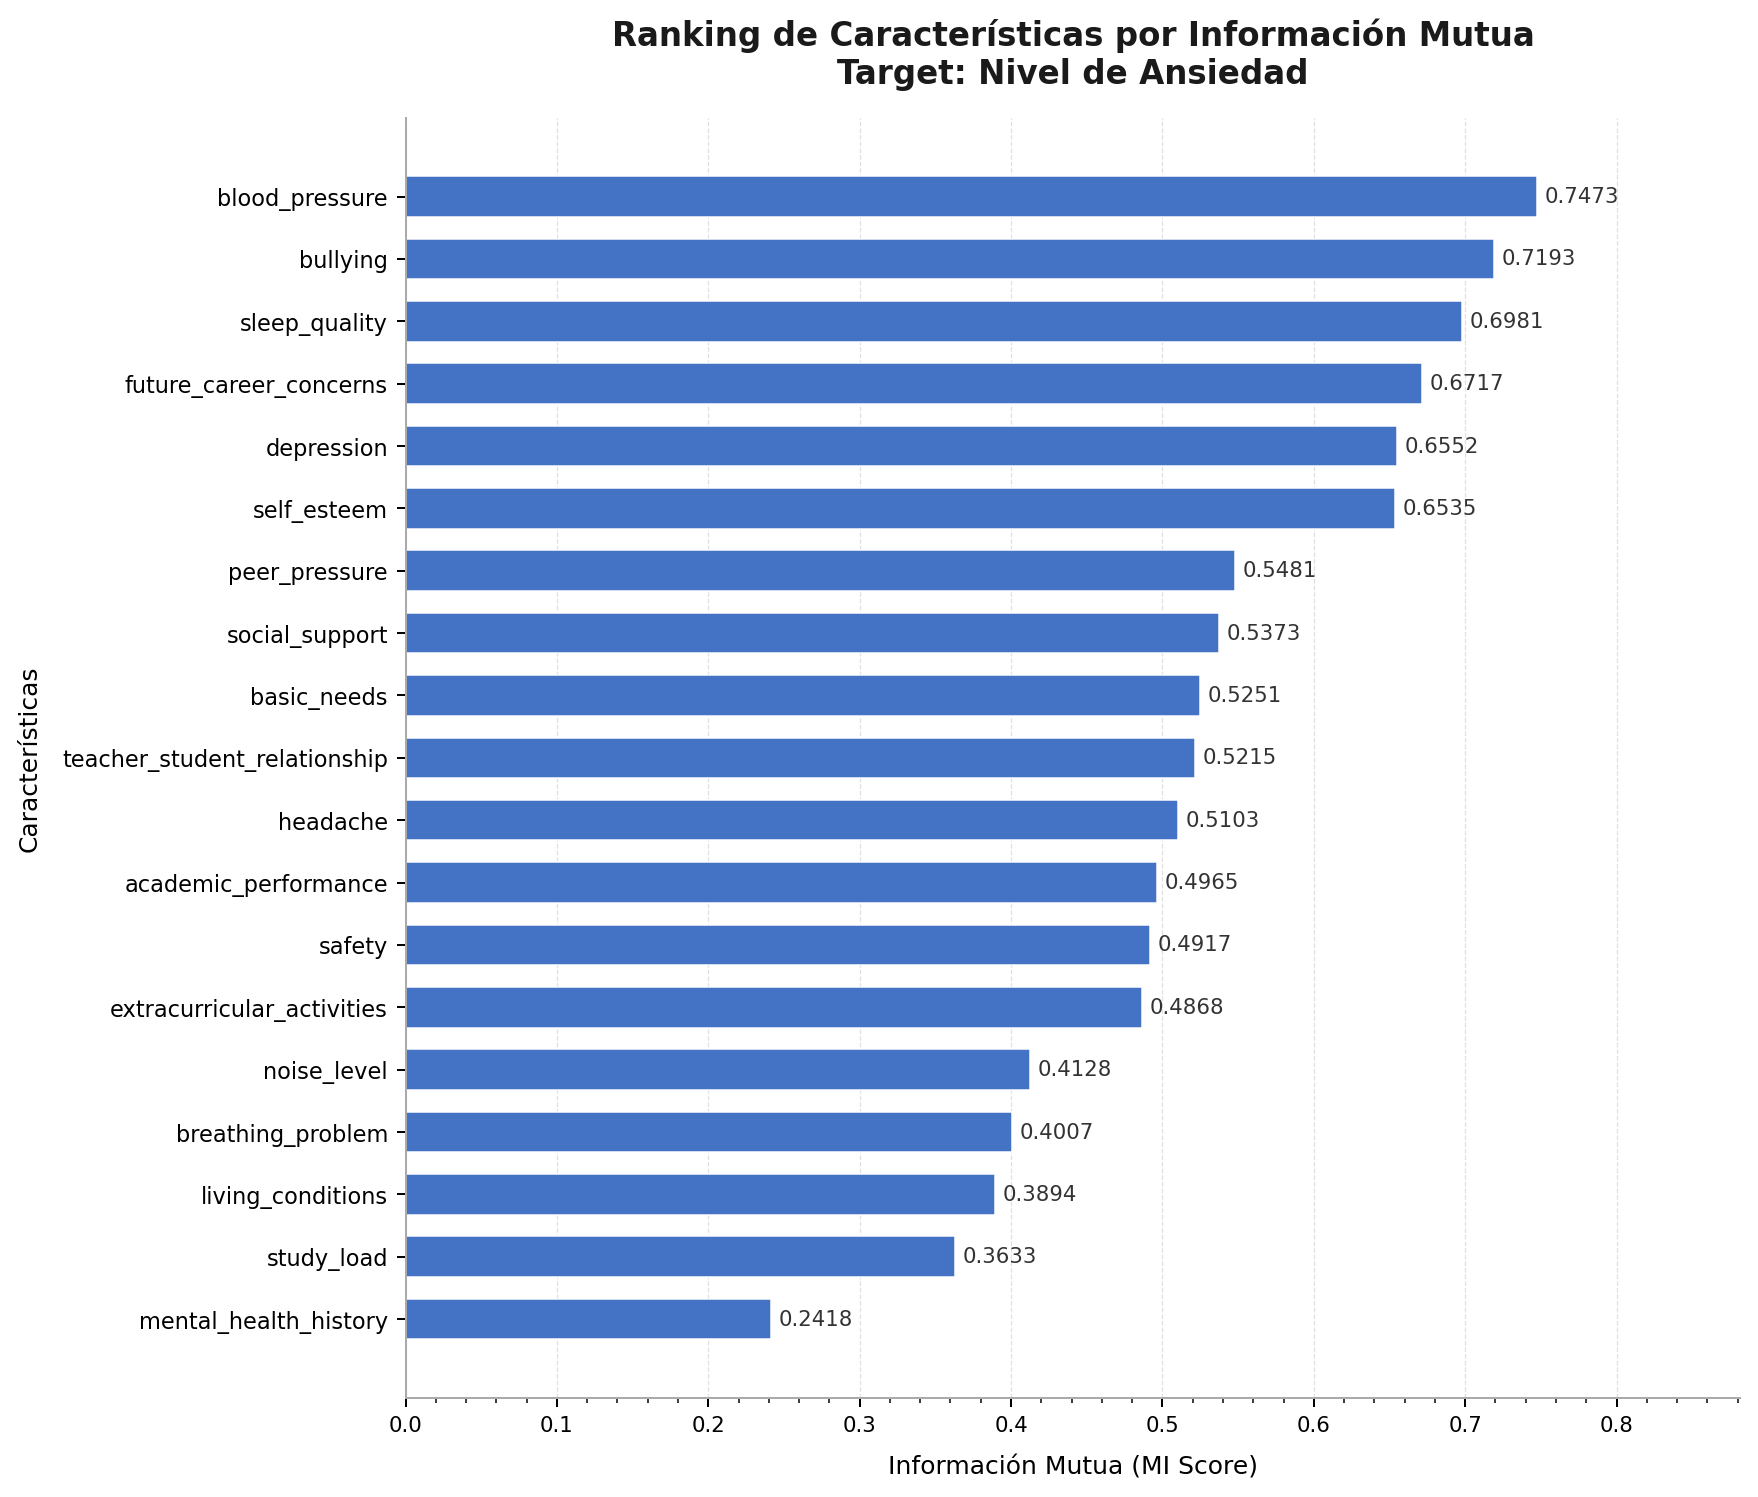
\includegraphics[width=0.92\textwidth]{results/ranking_mmi_anxiety.png}
    \caption{Ranking de Información Mutua — Target: Nivel de Ansiedad}
    \label{fig:mmi_anxiety}
\end{figure}

% ── Figura 2: Depresión ─────────────────────────────────────────────────────
\begin{figure}[H]
    \centering
    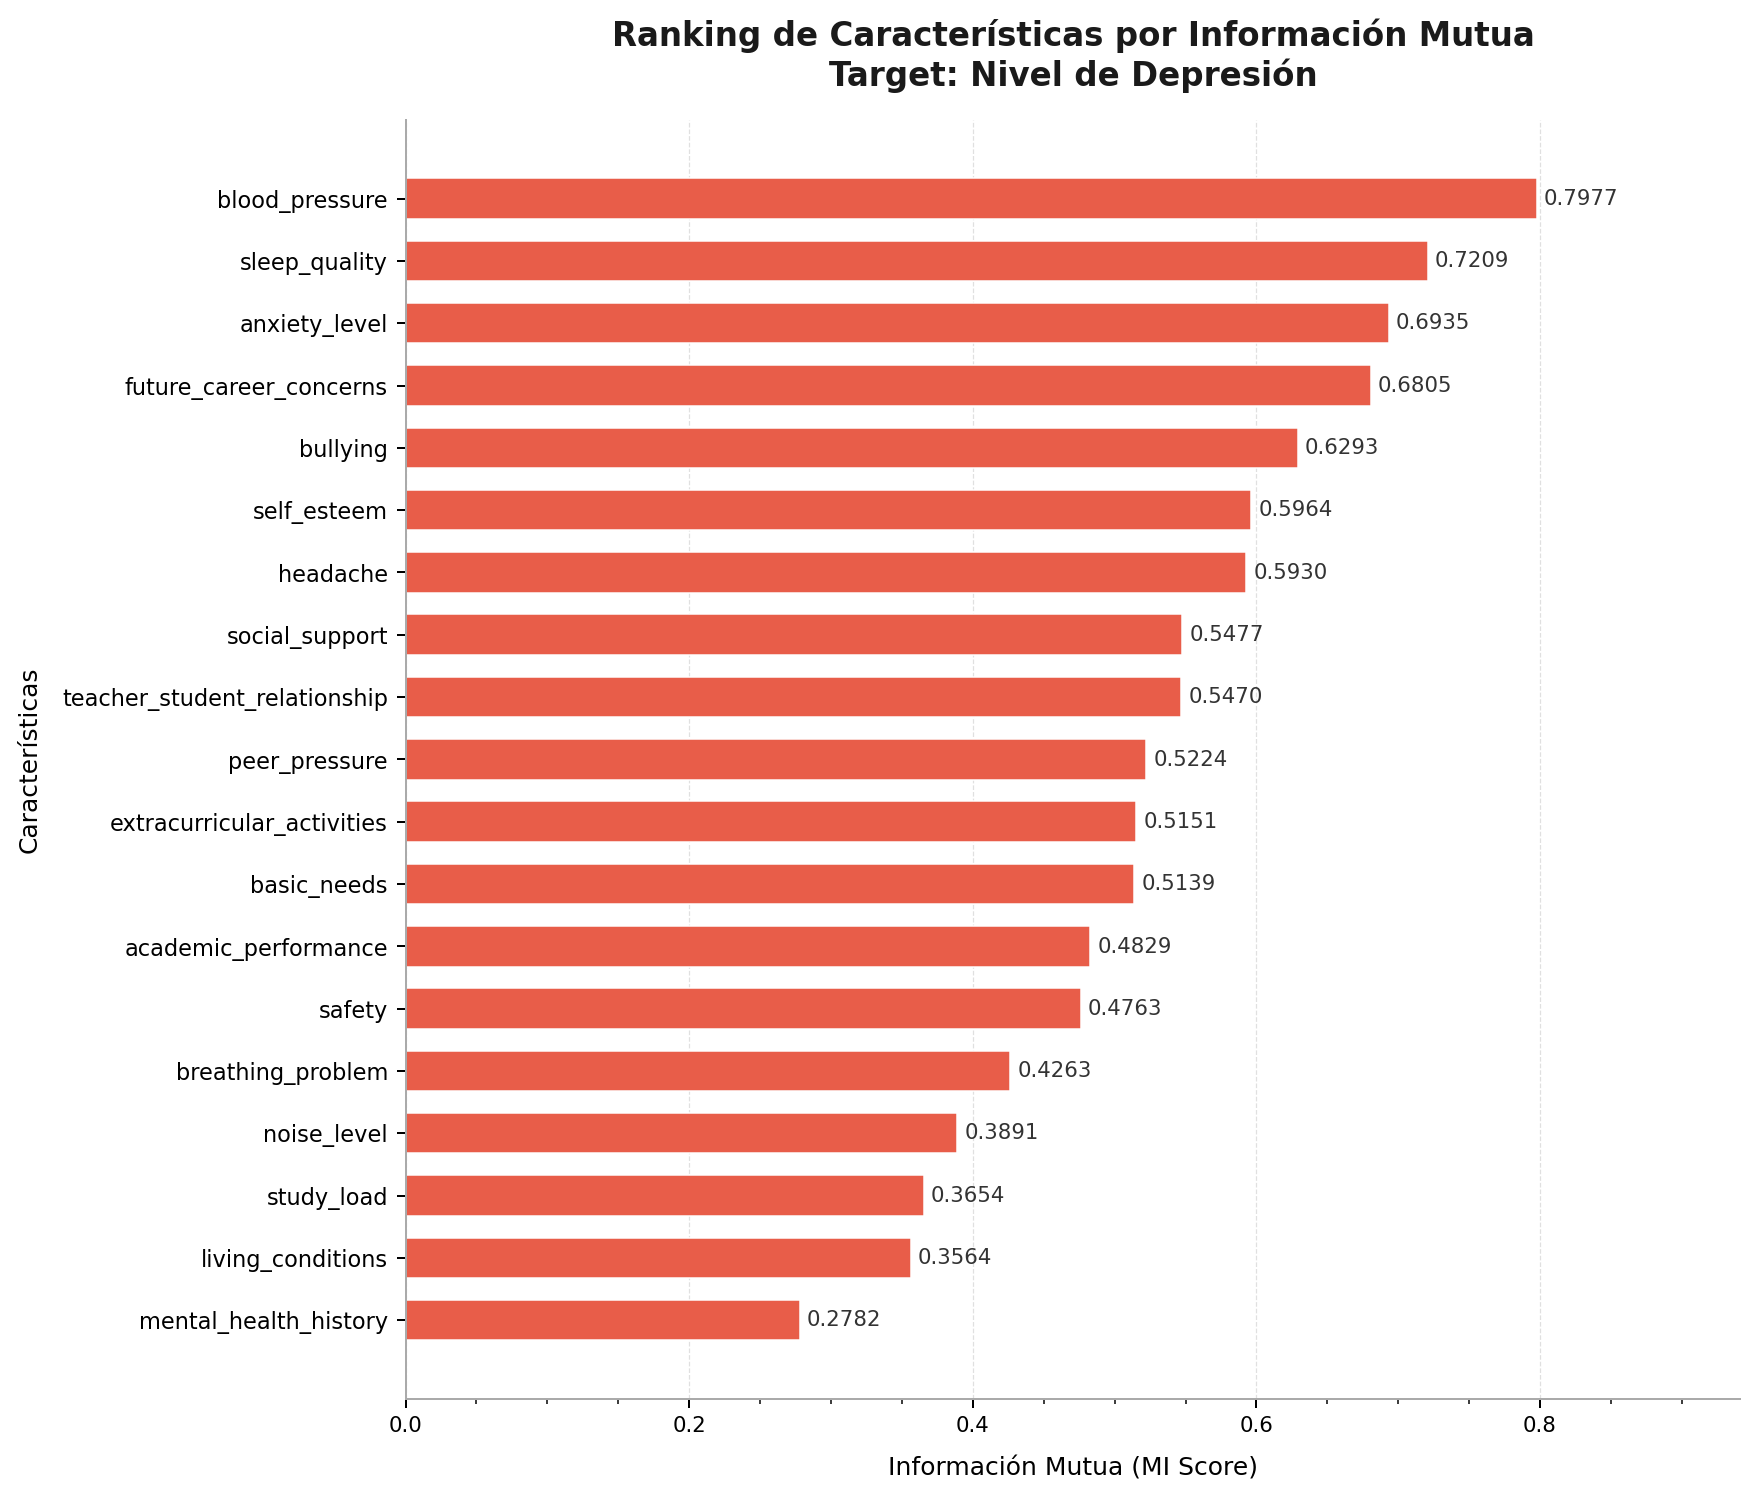
\includegraphics[width=0.92\textwidth]{results/ranking_mmi_depression.png}
    \caption{Ranking de Información Mutua — Target: Nivel de Depresión}
    \label{fig:mmi_depression}
\end{figure}

\subsection{Entrenamiento con Top-10 MMI}

Se seleccionaron las \textbf{10 variables} con mayor score MMI respecto a
\texttt{stress\_level} y se volvieron a entrenar ambos modelos. La
Tabla~\ref{tab:tarea2} muestra los resultados obtenidos.

\begin{table}[H]
    \centering
    \caption{Métricas de clasificación — Tarea 2 (Top-10 MMI)}
    \label{tab:tarea2}
    \begin{tabular}{lcccc}
        \toprule
        \textbf{Modelo} & \textbf{Accuracy} & \textbf{Precision} &
        \textbf{Recall} & \textbf{F1-Score} \\
        \midrule
        \rowcolor{rowgray}
        Gaussian Naive Bayes      & 87.27\% & 0.8943 & 0.8727 & 0.8752 \\
        Decision Tree (depth=6)   & 86.97\% & 0.8697 & 0.8697 & 0.8696 \\
        \bottomrule
    \end{tabular}
\end{table}

% ============================================================
\section{Análisis Comparativo de Resultados}
% ============================================================

La Tabla~\ref{tab:comparacion} consolida las métricas de ambas tareas para
facilitar la comparación directa entre el uso de todas las variables y el
subconjunto reducido por MMI.

\begin{table}[H]
    \centering
    \caption{Comparación Tarea 1 (todas las variables) vs.\ Tarea 2 (Top-10 MMI)}
    \label{tab:comparacion}
    \begin{tabular}{lcccc}
        \toprule
        \multirow{2}{*}{\textbf{Modelo}} &
        \multicolumn{2}{c}{\textbf{Accuracy}} &
        \multicolumn{2}{c}{\textbf{F1-Score (weighted)}} \\
        \cmidrule(lr){2-3}\cmidrule(lr){4-5}
        & \textbf{Tarea 1} & \textbf{Tarea 2} &
          \textbf{Tarea 1} & \textbf{Tarea 2} \\
        \midrule
        \rowcolor{rowgray}
        Gaussian Naive Bayes     & 88.18\% & 87.27\% & 0.8837 & 0.8752 \\
        Decision Tree (depth=6)  & 88.48\% & 86.97\% & 0.8849 & 0.8696 \\
        \bottomrule
    \end{tabular}
\end{table}

Los resultados muestran que la reducción del 50\% de las variables
(de 20 a 10) provocó una disminución de exactitud de únicamente:

\begin{itemize}
    \item $\Delta\,\text{Acc}_{\text{NB}} = -0.91\%$
    \item $\Delta\,\text{Acc}_{\text{DT}} = -1.51\%$
\end{itemize}

Este resultado confirma que las 10 variables descartadas aportaban
información redundante o de baja discriminancia, y que el ranking
MMI identificó correctamente el núcleo informativo del dataset.

\subsection{Hallazgo central: \texttt{blood\_pressure} como predictor universal}

La variable \texttt{blood\_pressure} obtuvo el \textbf{primer lugar} en los
tres rankings calculados (stress, ansiedad y depresión), con scores MMI
superiores a 0.74 en todos los casos. Esto sugiere que la presión arterial
es el indicador fisiológico más fuertemente correlacionado con el bienestar
mental en esta muestra estudiantil, lo que es coherente con la literatura
médica sobre la conexión entre el sistema nervioso autónomo y los estados
de estrés crónico.

% ============================================================
\section{Conclusiones}
% ============================================================

A partir del análisis realizado se derivan las siguientes conclusiones:

\begin{enumerate}

    \item \textbf{Alta precisión base.}
    Ambos modelos, Gaussian Naive Bayes y Decision Tree, alcanzan más del
    \textbf{88\%} de exactitud con las 20 variables completas, demostrando
    que el dataset presenta patrones de clase bien definidos y separables.

    \item \textbf{Robustez ante reducción de dimensionalidad.}
    La selección por Información Mutua permitió reducir el espacio de
    características en un \textbf{50\%} con una caída máxima de exactitud
    de apenas \textbf{1.5\%} (Decision Tree). Este resultado valida la
    eficiencia del ranking MMI como método de selección de características
    para datos discretos y ordinales.

    \item \textbf{Recall destacado en detección de estrés alto.}
    Gaussian Naive Bayes mantuvo un Recall de \textbf{96\%} para la clase
    \textit{Alto (2)} en ambas tareas, propiedad crítica para aplicaciones
    de detección temprana donde un falso negativo tiene mayor costo que
    un falso positivo.

    \item \textbf{Superioridad de MMI sobre Fisher para datos ordinales.}
    El contraste entre ambos métodos de ranking reveló discrepancias
    significativas (p.~ej., \texttt{academic\_performance}: Fisher \#4 vs.
    MMI \#13), confirmando que el Factor de Fisher sobrevalora variables
    con alta separación lineal de medias pero baja capacidad discriminante
    no lineal.

    \item \textbf{Predictor universal: \texttt{blood\_pressure}.}
    Esta variable lideró los tres rankings de importancia (stress, ansiedad
    y depresión), posicionándose como el predictor fisiológico central del
    bienestar mental en el contexto estudiantil analizado.

\end{enumerate}

% ============================================================
\newpage
\begin{thebibliography}{9}

\bibitem{mitchell1997}
    Mitchell, T.~M. (1997).
    \textit{Machine Learning}.
    McGraw-Hill.

\bibitem{sklearn}
    Pedregosa, F. et al. (2011).
    Scikit-learn: Machine Learning in Python.
    \textit{Journal of Machine Learning Research}, 12, 2825--2830.

\bibitem{cover2006}
    Cover, T.~M. \& Thomas, J.~A. (2006).
    \textit{Elements of Information Theory} (2a ed.).
    Wiley-Interscience.

\bibitem{quinlan1986}
    Quinlan, J.~R. (1986).
    Induction of Decision Trees.
    \textit{Machine Learning}, 1(1), 81--106.

\bibitem{shannon1948}
    Shannon, C.~E. (1948).
    A Mathematical Theory of Communication.
    \textit{Bell System Technical Journal}, 27, 379--423.

\end{thebibliography}

\end{document}
